\section{Roadmap and Timeline} \label{sec:timeline}

Table~\ref{tab:milestones} provides a list of key milestones for Rubin Operations and the Early Science Program.
It will continue to be updated as Rubin Construction and the Early Science Program progress. 
The date ranges are derived from the Rubin ``Celebratory Milestones'', which are  published monthly on the Rubin Project website\footnote{\url{https://www.lsst.org/about/project-status}}. 

\begin{table}[ht]
\centering
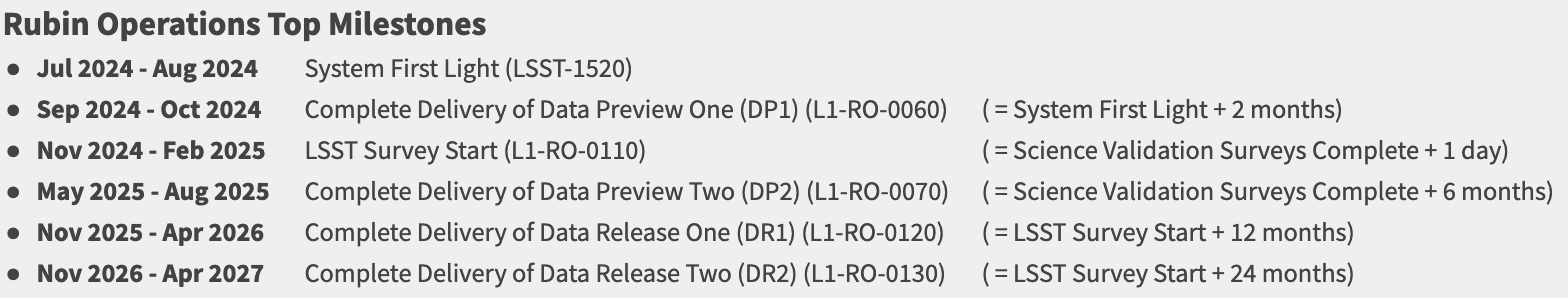
\includegraphics[width=\linewidth]{figures/DPR-milestones}
\caption{Top milestones for the Early Science Program.}
\label{tab:milestones}
\end{table}

Milestone dates are given as min-max ranges to indicate the associated uncertainty. 
Typically the near date corresponds to the current Project forecast, plus any additional operational uncertainty.
The late date corresponds (approximately) to the current Project ``late date'' plus any additional operational uncertainty and cannot be surpassed without the Project re-baselining its schedule.
An intermediate (typically mid-range) date is used by the Rubin Operations teams for planning purposes. 

The LSST survey will start shortly after the completion of the SV surveys, currently expected to be sometime between February 2025 and September 2025.
The timing of the Commissioning observations is somewhat less uncertain and the timing of the release of those data to the community can be projected to within a few months at the time of writing.

Table \ref{tab:timeline} shows the nominal date ranges for the various elements of the Early Science Program. 
The next key milestone in the Early Science Program is the release of DP0.3. 
Scheduled for mid-2023, DP0.3 will be the last in the DP0 series, which is based on simulated LSST-like data. 
The late dates for the DP2 and DR1 milestones allow for the possibility that the Project completes within its late date, but in doing so reduces the amount of on-sky LSSTCam commissioning time.
In this eventuality, the operations team would spend up to 3 months prior to commencing the 10-year LSST survey completing any remaining SV Survey observations , such that DP2 could be realized as planned.

\begin{table}[ht]
\centering
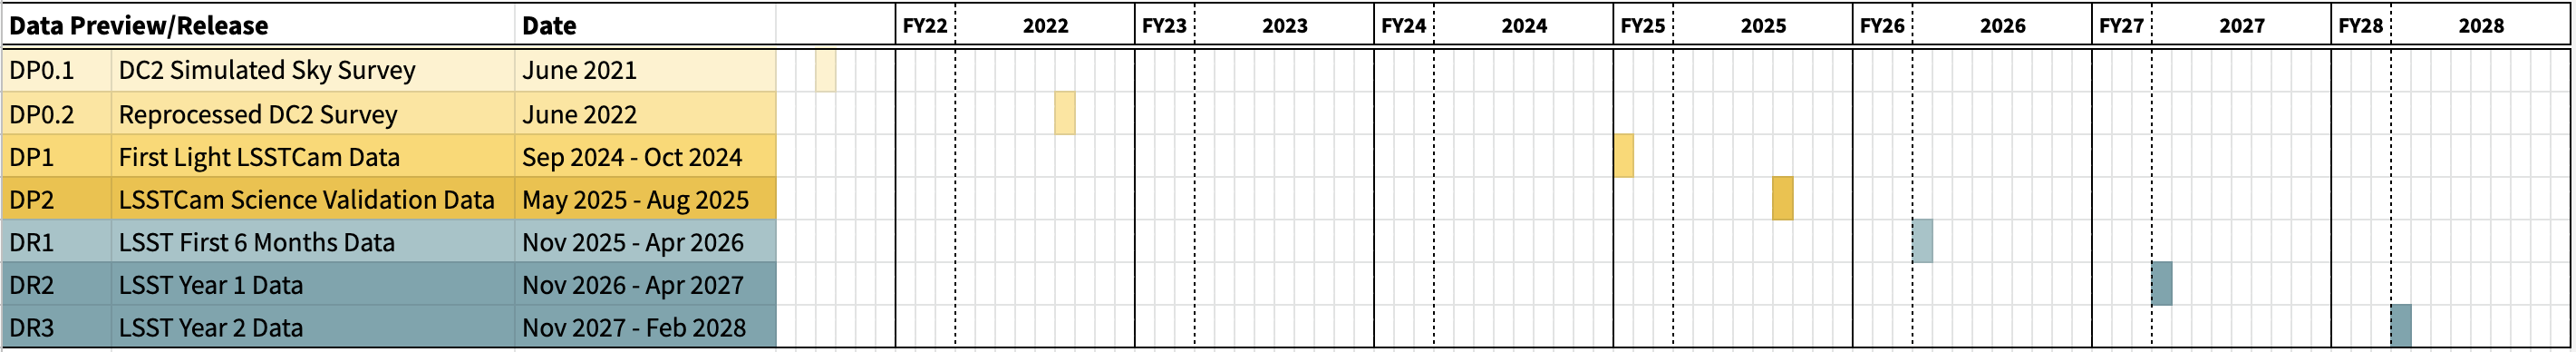
\includegraphics[width=\linewidth]{figures/DPR-timeline}
\caption{Nominal dates ranges for the various elements of the Early Science Program.}
\label{tab:timeline}
\end{table}

Tables ~\ref{tab:milestones} and ~\ref{tab:timeline} will continue to be refined and updated in future version of this documents as the Early Science Program progresses.
